\documentclass[12pt, logo=tehranDLDL/ut]{tehranDLDL}
\usepackage{pgfplots}
\usepackage{todonotes}
\usepackage[american, siunitx]{circuitikz}
\usepackage{tikz-timing}

\suptitle{Experiment 2}
\supsubtitle{Sessions 4, 5}
\title{Frequency Regulation}
\author{Katayoon Basharkhah \& Hadi Safari}
\preparer{Katayoon Basharkhah}
\supervisor{Professor Z. Navabi}
\university{University of Tehran}
\college{College of Engineering\\School of Electrical \& Computer Engineering}
\course[DLLab]{Digital Logic Laboratory}
\coursecode{ECE 045}
\courseurl{https://gitlab.com/hadi_sfr/ut-dldlab/-/jobs/artifacts/master/download?job=build}
\date{Spring 1398}

\graphicspath{{img/2/}}
\usetikzlibrary{positioning, shapes.multipart, shapes, arrows.meta}
\pgfplotsset{compat=1.16}

\begin{document}

\maketitle

\tableofcontents
\newpage

\section*{Introduction}
\addcontentsline{toc}{section}{Introduction}

Synchronization is a crucial issue in sequential digital circuit design. Many electrical devices devote multiple internal clocks to synchronize the internal processes. As you got familiar with the clock generation concepts in the previous experiment, it is consisted of a reference clock generator, like a ring oscillator, that is desired to output a stable reference clock by putting an odd number of inverters in a loop chain. However, the thermal variation of the oscillator causes variations in the clock frequency and this ruins the calculations in a digital processor.

The goal of this experiment is to design an adjustable clock generator that can fix the output frequency at the desired value. You will work on the interface between the FPGA and the external breadboard. You will learn how to consider the hardware design to make it a synthesizable one.

By the end of this experiment, you should have learned:
\begin{itemize}
    \item The concept of adjusting clock frequency
    \item Hardware implementation 
    \item Writing test-bench and simulation
\end{itemize}

The block diagram of the clock adjustment system is shown in \fref{fig:clock_adj}. It is consisted of two parts:
The first one is the circuit used in the previous experiment including a ring oscillator and a counter for frequency division.
The second part is a processing element that receives the output of the counter and sets its frequency to a specific value via a feedback path.
In fact, the processor changes the value that the oscillator is generating by dividing it by either a larger or a smaller value.

After constructing the clock generator circuit on the breadboard, you are to write a Verilog code for the processing element in FPGA.
First, you should model system behavior in Modelsim by writing an accurate hardware model in simulation and, after model verification, you should set the interface between the breadboard and FPGA.

\begin{figure}
    \centering
    \caption{Clock adjusting system\label{fig:clock_adj}}
    \resizebox{0.9\textwidth}{!}{
    \begin{circuitikz}
        % left
        \draw[thick, fill={Black!10!White}] (0,0) rectangle (7,3);
        \node at (3.5,2) {\Large 74LS191};
        \node at (3.5,1) {\Large LSB};
        \draw (1,3) -- ++(0,1) node[vcc] {};
        \draw (1,0) -- ++(0,-1) node[ground] {};
        \node[ocirc,scale=2] (lsb-ld) at (2,3) {};
        \draw (3,3) -- ++(0,1) node[circ] {} -- (3.97, 4.975);
        \draw (4,3) -- ++(0,1) node[circ] {} -- (4.20, 4.975);
        \draw (5,3) -- ++(0,1) node[circ] {} -- (4.92, 4.975);
        \draw (6,3) -- ++(0,1) node[circ] {} -- (5.15, 4.975);
        \draw (3,0) -- ++(0,-1) node[circ] {};
        \draw (4,0) -- ++(0,-1) node[circ] {};
        \draw (5,0) -- ++(0,-1) node[circ] {};
        \draw (6,0) -- ++(0,-1) node[circ] {};
        \node[ocirc,scale=2] (lsb-rclk) at (7,1) {};
        \node at (6,1) {ripple clock};
        \node at (6,2) {max/min};
        \node at (0.5,2) {clock};
        \node at (2,2.75) {load};
        \node at (3,2.75) {$A$};
        \node at (4,2.75) {$B$};
        \node at (5,2.75) {$C$};
        \node at (6,2.75) {$D$};
        \node at (3,0.25) {$Q_A$};
        \node at (4,0.25) {$Q_B$};
        \node at (5,0.25) {$Q_C$};
        \node at (6,0.25) {$Q_D$};
        % right
        \draw[thick, fill={Black!10!White}] (9,0) rectangle (16,3);
        \node at (12.5,2) {\Large 74LS191};
        \node at (12.5,1) {\Large MSB};
        \draw (9+1,3) -- ++(0,1) node[vcc] {};
        \draw (9+1,0) -- ++(0,-1) node[ground] {};
        \node[ocirc,scale=2] (msb-ld) at (9+2,3) {};
        \draw (9+3,3) -- ++(0,1) node[circ] {} -- (12.98, 4.975);
        \draw (9+4,3) -- ++(0,1) node[circ] {} -- (13.2, 4.975);
        \draw (9+5,3) -- ++(0,1) node[circ] {} -- (13.92, 4.975);
        \draw (9+6,3) -- ++(0,1) node[circ] {} -- (14.17, 4.975);
        \draw (9+3,0) -- ++(0,-1) node[circ] {};
        \draw (9+4,0) -- ++(0,-1) node[circ] {};
        \draw (9+5,0) -- ++(0,-1) node[circ] {};
        \draw (9+6,0) -- ++(0,-1) node[circ] {};
        \node[ocirc,scale=2] (msb-rclk) at (9+7,1) {};
        \node at (9+6,1) {ripple clock};
        \node at (9+6,2) {max/min};
        \node at (9+0.5,2) {clock};
        \node at (9+2,2.75) {load};
        \node at (9+3,2.75) {$A$};
        \node at (9+4,2.75) {$B$};
        \node at (9+5,2.75) {$C$};
        \node at (9+6,2.75) {$D$};
        \node at (9+3,0.25) {$Q_A$};
        \node at (9+4,0.25) {$Q_B$};
        \node at (9+5,0.25) {$Q_C$};
        \node at (9+6,0.25) {$Q_D$};
        % wiring
        \draw (7,2) -- (9+0,2);
        \draw (msb-rclk) -| ++(1,3.75) -| (msb-ld);
        \draw (msb-rclk) -| ++(1,3.75) -| (lsb-ld);
        \node[vsourcesquareshape, scale=1.5, label={ring oscillator}] (src) at (-2,2) {};
        \draw (src.right) -- (0,2);
        \draw (9+7,2) -| (18.4,8.65);
        \draw (17.28,6.86) -- ++(0, -0.1) -| (17.8,8.65);
        \draw[-{latex}] (17.28,8.06) -- +(0,0.1) -- (14.3-3.5,8.06);
        \node[anchor=west] at (14.3-3.5+0.1,8.06+0.25) {PSI};
        \draw[{latex}-] (14.17, 6.18) |- (14.3-3.5, -3.75+11);
        \draw[{latex}-] (13.92, 6.18) |- (14.3-3.5, -4+11);
        \draw[{latex}-] (13.2, 6.18) |- (14.3-3.5, -4.25+11);
        \draw[{latex}-] (12.98, 6.18) |- (14.3-3.5, -4.5+11);
        \node[anchor=west] at (14.3-3.5+0.1, -3.75+11+0.25) {adjustedDiv[7:4]};
        \draw[{latex}-] (3.97, 6.18) |- (10-3.5, -3.75+11);
        \draw[{latex}-] (4.20, 6.18) |- (10-3.5, -4+11);
        \draw[{latex}-] (4.92, 6.18) |- (10-3.5, -4.25+11);
        \draw[{latex}-] (5.15, 6.18) |- (10-3.5, -4.5+11);
        \node[anchor=east] at (10-3.5-0.1, -3.75+11+0.25) {adjustedDiv[3:0]};
        % FPGA
        \draw[thick, fill={Black!10!White}] (10-3.5,5.1) rectangle (14.3-3.5,9.1);
        \node at (12.15-3.5,6.6) {\Large FPGA};
        \draw[fill=Blue] (10.6-3.5,7.8) rectangle (13.7-3.5,8.8);
        \draw[Cerulean,very thick] (10.8+0.15+0.01-3.5,8.0) rectangle ++(0.4,0.02);
        \draw[Cerulean,very thick] (10.8+0.15+0.01-3.5,8.3) rectangle ++(0.4,0.02);
        \draw[Cerulean,very thick] (10.8+0.15+0.01-3.5,8.6) rectangle ++(0.4,0.02);
        \draw[Cerulean,very thick] (11.78+0.15+0.01-3.5,8.0) rectangle ++(0.4,0.02);
        \draw[Cerulean,very thick] (11.78+0.15+0.01-3.5,8.3) rectangle ++(0.4,0.02);
        \draw[Cerulean,very thick] (11.78+0.15+0.01-3.5,8.6) rectangle ++(0.4,0.02);
        \draw[Cerulean,very thick] (12.8+0.15+0.01-3.5,8.0) rectangle ++(0.4,0.02);
        \draw[Cerulean,very thick] (12.8+0.15+0.01-3.5,8.3) rectangle ++(0.4,0.02);
        \draw[Cerulean,very thick] (12.8+0.15+0.01-3.5,8.6) rectangle ++(0.4,0.02);
        \draw[Cerulean,very thick] (10.72+0.15-3.5,8.050) rectangle ++(0.02,0.2);
        \draw[Cerulean,very thick] (10.72+0.15-3.5,8.375) rectangle ++(0.02,0.2);
        \draw[Cerulean,very thick] (11.28+0.15-3.5,8.050) rectangle ++(0.02,0.2);
        \draw[Cerulean,very thick] (11.28+0.15-3.5,8.375) rectangle ++(0.02,0.2);
        \draw[Cerulean,very thick] (11.70+0.15-3.5,8.050) rectangle ++(0.02,0.2);
        \draw[Cerulean,very thick] (11.70+0.15-3.5,8.375) rectangle ++(0.02,0.2);
        \draw[Cerulean,very thick] (12.26+0.15-3.5,8.050) rectangle ++(0.02,0.2);
        \draw[Cerulean,very thick] (12.26+0.15-3.5,8.375) rectangle ++(0.02,0.2);
        \draw[Cerulean,very thick] (12.72+0.15-3.5,8.050) rectangle ++(0.02,0.2);
        \draw[Cerulean,very thick] (12.72+0.15-3.5,8.375) rectangle ++(0.02,0.2);
        \draw[Cerulean,very thick] (13.28+0.15-3.5,8.050) rectangle ++(0.02,0.2);
        \draw[Cerulean,very thick] (13.28+0.15-3.5,8.375) rectangle ++(0.02,0.2);
        % \node at (7-3.5,5.1) {duration of divided clock};
        % \draw[<-] (7-3.5,5.3) to[bend left] (10.15-3.5,6.55);
        \begin{scope}[scale=0.1, shift={(175,95)}, rotate=-90]
            % border
            \draw[thick, fill={Black!10!White}] (0,14) |- (7,0) |- (5,14) -- (4.5,14) arc(0:-180:1) -- cycle;
            \node at (3.5,7) {74LS74};
            % PINs
            \draw (0,0.25) rectangle (-1.5,1.75);
            \draw (0,2.25) rectangle (-1.5,3.75);
            \draw (0,4.25) rectangle (-1.5,5.75);
            \draw (0,6.25) rectangle (-1.5,7.75);
            \draw (0,8.25) rectangle (-1.5,9.75);
            \draw (0,10.25) rectangle (-1.5,11.75);
            \draw (0,12.25) rectangle (-1.5,13.75);
            \draw (7,0.25) rectangle (8.5,1.75);
            \draw (7,2.25) rectangle (8.5,3.75);
            \draw (7,4.25) rectangle (8.5,5.75);
            \draw (7,6.25) rectangle (8.5,7.75);
            \draw (7,8.25) rectangle (8.5,9.75);
            \draw (7,10.25) rectangle (8.5,11.75);
            \draw (7,12.25) rectangle (8.5,13.75);
        \end{scope}
        % level converter
        \begin{scope}[scale=0.12, shift={(135,65.7)}, rotate=-90]
            % border
            \draw[very thick, fill={Black!10!White}] (0,12) |- (7,0) |- (5,12) -- (4.5,12) arc(0:-180:1) -- cycle;
            \node at (2,6) {\tiny Voltage};
            \node at (3.5,6) {\tiny Level};
            \node at (5,6) {\tiny Converter};
            % PINs
            \draw (0,0.25) rectangle (-1.5,1.75);
            \draw (0,2.25) rectangle (-1.5,3.75);
            \draw (0,4.25) rectangle (-1.5,5.75);
            \draw (0,6.25) rectangle (-1.5,7.75);
            \draw (0,8.25) rectangle (-1.5,9.75);
            \draw (0,10.25) rectangle (-1.5,11.75);
            \draw (7,0.25) rectangle (8.5,1.75);
            \draw (7,2.25) rectangle (8.5,3.75);
            \draw (7,4.25) rectangle (8.5,5.75);
            \draw (7,6.25) rectangle (8.5,7.75);
            \draw (7,8.25) rectangle (8.5,9.75);
            \draw (7,10.25) rectangle (8.5,11.75);
        \end{scope}
        % level converter
        \begin{scope}[scale=0.12, shift={(107,50)}, rotate=-90]
            % border
            \draw[very thick, fill={Black!10!White}] (0,12) |- (7,0) |- (5,12) -- (4.5,12) arc(0:-180:1) -- cycle;
            \node at (2,6) {\tiny Voltage};
            \node at (3.5,6) {\tiny Level};
            \node at (5,6) {\tiny Converter};
            % PINs
            \draw (0,0.25) rectangle (-1.5,1.75);
            \draw (0,2.25) rectangle (-1.5,3.75);
            \draw (0,4.25) rectangle (-1.5,5.75);
            \draw (0,6.25) rectangle (-1.5,7.75);
            \draw (0,8.25) rectangle (-1.5,9.75);
            \draw (0,10.25) rectangle (-1.5,11.75);
            \draw (7,0.25) rectangle (8.5,1.75);
            \draw (7,2.25) rectangle (8.5,3.75);
            \draw (7,4.25) rectangle (8.5,5.75);
            \draw (7,6.25) rectangle (8.5,7.75);
            \draw (7,8.25) rectangle (8.5,9.75);
            \draw (7,10.25) rectangle (8.5,11.75);
        \end{scope}
        % level converter
        \begin{scope}[scale=0.12, shift={(32,50)}, rotate=-90]
            % border
            \draw[very thick, fill={Black!10!White}] (0,12) |- (7,0) |- (5,12) -- (4.5,12) arc(0:-180:1) -- cycle;
            \node at (2,6) {\tiny Voltage};
            \node at (3.5,6) {\tiny Level};
            \node at (5,6) {\tiny Converter};
            % PINs
            \draw (0,0.25) rectangle (-1.5,1.75);
            \draw (0,2.25) rectangle (-1.5,3.75);
            \draw (0,4.25) rectangle (-1.5,5.75);
            \draw (0,6.25) rectangle (-1.5,7.75);
            \draw (0,8.25) rectangle (-1.5,9.75);
            \draw (0,10.25) rectangle (-1.5,11.75);
            \draw (7,0.25) rectangle (8.5,1.75);
            \draw (7,2.25) rectangle (8.5,3.75);
            \draw (7,4.25) rectangle (8.5,5.75);
            \draw (7,6.25) rectangle (8.5,7.75);
            \draw (7,8.25) rectangle (8.5,9.75);
            \draw (7,10.25) rectangle (8.5,11.75);
        \end{scope}
    \end{circuitikz}
    }
\end{figure}

\section{Design Description and Simulation}

The goal of the design is to receive the output of frequency divider and set the output frequency at a fixed value. To do this, a design like \fref{fig:clock_adj} is needed. The processor should calculate the input frequency and compare it with a reference signal. If the reference and the input’s frequencies are not the same, then it should change the division value. So, the load inputs of the counter should be fed to the FPGA and must be increased or decreased whether the frequency is higher or lower than the reference value.

\begin{figure}[b]
    \caption{Frequency regulator pins\label{fig:freq_reg}}
    \centering
    \resizebox{0.6\textwidth}{!}{
    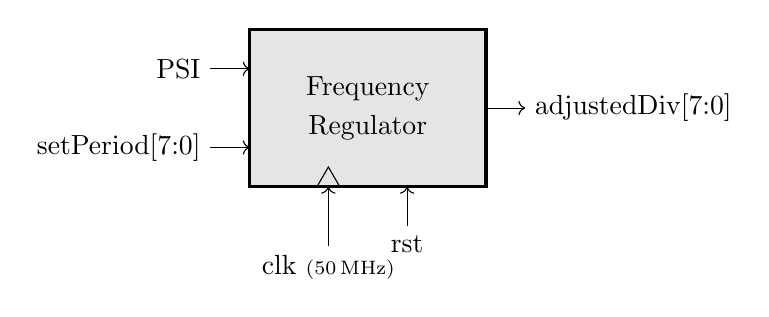
\begin{tikzpicture}
        \draw[very thick,fill={Black!10!White}] (0,0) rectangle (3,2);
        \node at (1.5,1.25) {Frequency};
        \node at (1.5,0.75) {Regulator};
        \draw[<-] (0,0.5) to ++(-0.5,0) node[left] {\lstinline{setPeriod[7:0]}};
        % \draw[<-] (0,1) to ++(-0.5,0) node[left] {\lstinline{presentDiv[7:0]}};
        \draw[<-] (0,1.5) to ++(-0.5,0) node[left] {\lstinline{PSI}};
        \draw[->] (3,1) to ++(0.5,0) node[right] {\lstinline{adjustedDiv[7:0]}};
        \draw[<-] (2,0) to ++(0,-0.5) node[below] {\lstinline{rst}};
        \draw[<-] (1,0) to ++(0,-0.75) node[below] {\lstinline{clk} \scriptsize(\SI{50}{\mega\hertz})};
        \node[draw, regular polygon, regular polygon sides=3, scale=0.5, anchor=south] at (1,0) {};
    \end{tikzpicture}
    }
\end{figure}

DE1 board works with a \SI{50}{\mega\hertz} clock frequency that is definitely much higher than the input frequency. When the input comes in, FPGA starts to count its duration by this clock at the input rising edge and stops counting by the falling edge.

The inputs and outputs of the design are shown in \fref{fig:freq_reg}. The adjusted value for division after processing is called \lstinline{adjustedDiv}. The reference value called \lstinline{setPeriod} is also another input that shows the ratio of the FPGA clock and the input signal. \lstinline{PSI}, the divided clock after passing flip-flop, is the main input of FPGA and frequency regulation will be performed based on it.

To measure the input frequency, a counter starts to count the signal duration when the input signal gets 1. When the input goes to 0, the counter stops counting and the last value of the counter will be stored in a register. At the rise edge of the input signal, the counter value will be reset.
Use an \lstinline{always} statement like below to determine the duration value. You can use a \lstinline{case} statement to set the duration value at 4 states described above:
\begin{lstlisting}
always @(posedge clk, posedge rst) begin : decide_when_to_count_and_count
    if (rst)
        // ...
    else begin
        case (/* input signal transition */)
            // zero to one
            // steady at one
            // one to zero
            // steady at zero
        endcase
    end
end
\end{lstlisting}

The comparison must be performed when the input is at 0. Frequency adjustment will be performed by an increment or decrement signal. When the duration is more than the reference value, the present value of the load inputs should be increased and if its value is less than the reference signal then the load inputs should be decreased. Hence an Increment and decrement signal should be set to 1 after the comparison.

Again, use an \lstinline{always} statement to change the increment and decrement value at the proper time:
\begin{lstlisting}
always @(/* input and count transition */) begin : comparison
    if (/* one to zero */) begin
        // comparison
        // set the inc and dec value
    end
end
\end{lstlisting}

When the comparison is completed, by the falling edge of the input signal and based on the increment or decrement value, the present value of the load inputs will be changed and registered to the adjusted value. The third \lstinline{always} block is dedicated to this performance:
\begin{lstlisting}
always @(posedge clk, posedge rst) begin : increment_decrement
    if (// one to zero //) begin
        // increment or decrement
    end
end
\end{lstlisting}

\begin{enumerate}
    \item Write a Verilog code based on this instructions.
    \item Provide a test-bench for you design and verify your design. Note that the test-bench is a high-level abstraction model of your design. Therefore, you should accurately model the real hardware inside your test-bench.
    \item Include all the simulation results, the Quartus~II project and the simulation waveforms in your report.
\end{enumerate}

\designverification{}

\section{Hardware Implementation}

After verifying your design, you should implement the hardware. Construct the circuit of \fref{fig:clock_adj}.  Since the division range of an 8-bit counter is wide, it is better to limit this range for observing the frequency regulation. To do this, you can just change the least-significant counter and set other four most-significant bits to a fixed number, which could be hard-wired or adjustable by DIP switches.

Consider two frequencies \SI{1.25}{\mega\hertz} and \SI{200}{\kilo\hertz} as examples. The parallel load for each of them is shown in the \fref{tab:par_load}. The four most-significant bits can be fixed on a breadboard with a dip switch. The connections for the load inputs are shown in \fref{fig:connections}.

\begin{figure}
    \centering
    \caption{Connections of the design\label{fig:connections}}
    \resizebox{0.9\textwidth}{!}{
    \begin{circuitikz}
        % left
        \draw[thick, fill={Black!10!White}] (0,0) rectangle (7,3);
        \node at (3.5,2) {\Large 74LS191};
        \node at (3.5,1) {\Large LSB};
        \draw (1,3) -- ++(0,1) node[vcc] {};
        \draw (1,0) -- ++(0,-1) node[ground] {};
        \node[ocirc,scale=2] (lsb-ld) at (2,3) {};
        \draw (3,3) -- ++(0,1) node[circ] {} -- (3.97, 4.975);
        \draw (4,3) -- ++(0,1) node[circ] {} -- (4.20, 4.975);
        \draw (5,3) -- ++(0,1) node[circ] {} -- (4.92, 4.975);
        \draw (6,3) -- ++(0,1) node[circ] {} -- (5.15, 4.975);
        \draw (3,0) -- ++(0,-1) node[circ] {};
        \draw (4,0) -- ++(0,-1) node[circ] {};
        \draw (5,0) -- ++(0,-1) node[circ] {};
        \draw (6,0) -- ++(0,-1) node[circ] {};
        \node[ocirc,scale=2] (lsb-rclk) at (7,1) {};
        \node at (6,1) {ripple clock};
        \node at (6,2) {max/min};
        \node at (0.5,2) {clock};
        \node at (2,2.75) {load};
        \node at (3,2.75) {$A$};
        \node at (4,2.75) {$B$};
        \node at (5,2.75) {$C$};
        \node at (6,2.75) {$D$};
        \node at (3,0.25) {$Q_A$};
        \node at (4,0.25) {$Q_B$};
        \node at (5,0.25) {$Q_C$};
        \node at (6,0.25) {$Q_D$};
        % right
        \draw[thick, fill={Black!10!White}] (9,0) rectangle (16,3);
        \node at (12.5,2) {\Large 74LS191};
        \node at (12.5,1) {\Large MSB};
        \draw (9+1,3) -- ++(0,1) node[vcc] {};
        \draw (9+1,0) -- ++(0,-1) node[ground] {};
        \node[ocirc,scale=2] (msb-ld) at (9+2,3) {};
        \draw (9+3,3) -- ++(0,0.35) node[circ] {} ++(0,1) node[circ] {} -- ++(0,1.2)  node[vdd] {};%node {} -- (12.98, 4.975);
        \draw (9+4,3) -- ++(0,0.35) node[circ] {} ++(0,1) node[circ] {} -- ++(0,1.2)  node[vdd] {};%node {} -- (13.2, 4.975);
        \draw (9+5,3) -- ++(0,0.35) node[circ] {} ++(0,1) node[circ] {} -- ++(0,1.2)  node[vdd] {};%node {} -- (13.92, 4.975);
        \draw (9+6,3) -- ++(0,0.35) node[circ] {} ++(0,1) node[circ] {} -- ++(0,1.2)  node[vdd] {};%node {} -- (14.17, 4.975);
        \node at (9+4.5,6.35) {$V_\mathit{CC}$~/~$\mathit{GND}$};
        \draw[fill={Black!10!White}] (9+3-0.5,3.35) rectangle ++(1,1);
        \draw[fill={Black!10!White}] (9+4-0.5,3.35) rectangle ++(1,1);
        \draw[fill={Black!10!White}] (9+5-0.5,3.35) rectangle ++(1,1);
        \draw[fill={Black!10!White}] (9+6-0.5,3.35) rectangle ++(1,1);
        \node[draw,circle,scale=2.5,fill=White,path picture={\node[toggleswitchshape,scale=0.9,shift={(0,-0.25)}] {};}] at (9+3,3.85) {};
        \node[draw,circle,scale=2.5,fill=White,path picture={\node[toggleswitchshape,scale=0.9,shift={(0,-0.25)}] {};}] at (9+4,3.85) {};
        \node[draw,circle,scale=2.5,fill=White,path picture={\node[toggleswitchshape,scale=0.9,shift={(0,-0.25)}] {};}] at (9+5,3.85) {};
        \node[draw,circle,scale=2.5,fill=White,path picture={\node[toggleswitchshape,scale=0.9,shift={(0,-0.25)}] {};}] at (9+6,3.85) {};
        \draw (9+3,0) -- ++(0,-1) node[circ] {};
        \draw (9+4,0) -- ++(0,-1) node[circ] {};
        \draw (9+5,0) -- ++(0,-1) node[circ] {};
        \draw (9+6,0) -- ++(0,-1) node[circ] {};
        \node[ocirc,scale=2] (msb-rclk) at (9+7,1) {};
        \node at (9+6,1) {ripple clock};
        \node at (9+6,2) {max/min};
        \node at (9+0.5,2) {clock};
        \node at (9+2,2.75) {load};
        \node at (9+3,2.75) {$A$};
        \node at (9+4,2.75) {$B$};
        \node at (9+5,2.75) {$C$};
        \node at (9+6,2.75) {$D$};
        \node at (9+3,0.25) {$Q_A$};
        \node at (9+4,0.25) {$Q_B$};
        \node at (9+5,0.25) {$Q_C$};
        \node at (9+6,0.25) {$Q_D$};
        % wiring
        \draw (7,2) -- (9+0,2);
        \draw (msb-rclk) -| ++(1,3.75) -| (msb-ld);
        \draw (msb-rclk) -| ++(1,3.75) -| (lsb-ld);
        \node[vsourcesquareshape, scale=1.5, label={ring oscillator}] (src) at (-2,2) {};
        \draw (src.right) -- (0,2);
        \draw (9+7,2) -| (18.4,8.65);
        \draw (17.28,6.86) -- ++(0, -0.1) -| (17.8,8.65);
        \draw[-{latex}] (17.28,8.06) -- +(0,0.1) -- (14.3-3.5,8.06);
        \node[anchor=west] at (14.3-3.5+0.1,8.06+0.25) {PSI};
        % \draw (14.17, 6.18) |- (14.3-3.5, -3.75+11);
        % \draw (13.92, 6.18) |- (14.3-3.5, -4+11);
        % \draw (13.2, 6.18) |- (14.3-3.5, -4.25+11);
        % \draw (12.98, 6.18) |- (14.3-3.5, -4.5+11);
        % \node[anchor=west] at (14.3-3.5+0.1, -3.75+11+0.25) {presentDiv[7:4]};
        \draw[{latex}-] (3.97, 6.18) |- (10-3.5, -3.75+11);
        \draw[{latex}-] (4.20, 6.18) |- (10-3.5, -4+11);
        \draw[{latex}-] (4.92, 6.18) |- (10-3.5, -4.25+11);
        \draw[{latex}-] (5.15, 6.18) |- (10-3.5, -4.5+11);
        \node[anchor=east] at (10-3.5-0.1, -3.75+11+0.25) {adjustedDiv[3:0]};
        % FPGA
        \draw[thick, fill={Black!10!White}] (10-3.5,5.1) rectangle (14.3-3.5,9.1);
        \node at (12.15-3.5,6.6) {\Large FPGA};
        \draw[fill=Blue] (10.6-3.5,7.8) rectangle (13.7-3.5,8.8);
        \draw[Cerulean,very thick] (10.8+0.15+0.01-3.5,8.0) rectangle ++(0.4,0.02);
        \draw[Cerulean,very thick] (10.8+0.15+0.01-3.5,8.3) rectangle ++(0.4,0.02);
        \draw[Cerulean,very thick] (10.8+0.15+0.01-3.5,8.6) rectangle ++(0.4,0.02);
        \draw[Cerulean,very thick] (11.78+0.15+0.01-3.5,8.0) rectangle ++(0.4,0.02);
        \draw[Cerulean,very thick] (11.78+0.15+0.01-3.5,8.3) rectangle ++(0.4,0.02);
        \draw[Cerulean,very thick] (11.78+0.15+0.01-3.5,8.6) rectangle ++(0.4,0.02);
        \draw[Cerulean,very thick] (12.8+0.15+0.01-3.5,8.0) rectangle ++(0.4,0.02);
        \draw[Cerulean,very thick] (12.8+0.15+0.01-3.5,8.3) rectangle ++(0.4,0.02);
        \draw[Cerulean,very thick] (12.8+0.15+0.01-3.5,8.6) rectangle ++(0.4,0.02);
        \draw[Cerulean,very thick] (10.72+0.15-3.5,8.050) rectangle ++(0.02,0.2);
        \draw[Cerulean,very thick] (10.72+0.15-3.5,8.375) rectangle ++(0.02,0.2);
        \draw[Cerulean,very thick] (11.28+0.15-3.5,8.050) rectangle ++(0.02,0.2);
        \draw[Cerulean,very thick] (11.28+0.15-3.5,8.375) rectangle ++(0.02,0.2);
        \draw[Cerulean,very thick] (11.70+0.15-3.5,8.050) rectangle ++(0.02,0.2);
        \draw[Cerulean,very thick] (11.70+0.15-3.5,8.375) rectangle ++(0.02,0.2);
        \draw[Cerulean,very thick] (12.26+0.15-3.5,8.050) rectangle ++(0.02,0.2);
        \draw[Cerulean,very thick] (12.26+0.15-3.5,8.375) rectangle ++(0.02,0.2);
        \draw[Cerulean,very thick] (12.72+0.15-3.5,8.050) rectangle ++(0.02,0.2);
        \draw[Cerulean,very thick] (12.72+0.15-3.5,8.375) rectangle ++(0.02,0.2);
        \draw[Cerulean,very thick] (13.28+0.15-3.5,8.050) rectangle ++(0.02,0.2);
        \draw[Cerulean,very thick] (13.28+0.15-3.5,8.375) rectangle ++(0.02,0.2);
        % \node at (7-3.5,5.1) {duration of divided clock};
        % \draw[<-] (7-3.5,5.3) to[bend left] (10.15-3.5,6.55);
        \begin{scope}[scale=0.1, shift={(175,95)}, rotate=-90]
            % border
            \draw[thick, fill={Black!10!White}] (0,14) |- (7,0) |- (5,14) -- (4.5,14) arc(0:-180:1) -- cycle;
            \node at (3.5,7) {74LS74};
            % PINs
            \draw (0,0.25) rectangle (-1.5,1.75);
            \draw (0,2.25) rectangle (-1.5,3.75);
            \draw (0,4.25) rectangle (-1.5,5.75);
            \draw (0,6.25) rectangle (-1.5,7.75);
            \draw (0,8.25) rectangle (-1.5,9.75);
            \draw (0,10.25) rectangle (-1.5,11.75);
            \draw (0,12.25) rectangle (-1.5,13.75);
            \draw (7,0.25) rectangle (8.5,1.75);
            \draw (7,2.25) rectangle (8.5,3.75);
            \draw (7,4.25) rectangle (8.5,5.75);
            \draw (7,6.25) rectangle (8.5,7.75);
            \draw (7,8.25) rectangle (8.5,9.75);
            \draw (7,10.25) rectangle (8.5,11.75);
            \draw (7,12.25) rectangle (8.5,13.75);
        \end{scope}
        % level converter
        \begin{scope}[scale=0.12, shift={(135,65.7)}, rotate=-90]
            % border
            \draw[very thick, fill={Black!10!White}] (0,12) |- (7,0) |- (5,12) -- (4.5,12) arc(0:-180:1) -- cycle;
            \node at (2,6) {\tiny Voltage};
            \node at (3.5,6) {\tiny Level};
            \node at (5,6) {\tiny Converter};
            % PINs
            \draw (0,0.25) rectangle (-1.5,1.75);
            \draw (0,2.25) rectangle (-1.5,3.75);
            \draw (0,4.25) rectangle (-1.5,5.75);
            \draw (0,6.25) rectangle (-1.5,7.75);
            \draw (0,8.25) rectangle (-1.5,9.75);
            \draw (0,10.25) rectangle (-1.5,11.75);
            \draw (7,0.25) rectangle (8.5,1.75);
            \draw (7,2.25) rectangle (8.5,3.75);
            \draw (7,4.25) rectangle (8.5,5.75);
            \draw (7,6.25) rectangle (8.5,7.75);
            \draw (7,8.25) rectangle (8.5,9.75);
            \draw (7,10.25) rectangle (8.5,11.75);
        \end{scope}
        % % level converter
        % \begin{scope}[scale=0.12, shift={(107,50)}, rotate=-90]
        %     % border
        %     \draw[very thick, fill={Black!10!White}] (0,12) |- (7,0) |- (5,12) -- (4.5,12) arc(0:-180:1) -- cycle;
        %     \node at (2,6) {\tiny Voltage};
        %     \node at (3.5,6) {\tiny Level};
        %     \node at (5,6) {\tiny Converter};
        %     % PINs
        %     \draw (0,0.25) rectangle (-1.5,1.75);
        %     \draw (0,2.25) rectangle (-1.5,3.75);
        %     \draw (0,4.25) rectangle (-1.5,5.75);
        %     \draw (0,6.25) rectangle (-1.5,7.75);
        %     \draw (0,8.25) rectangle (-1.5,9.75);
        %     \draw (0,10.25) rectangle (-1.5,11.75);
        %     \draw (7,0.25) rectangle (8.5,1.75);
        %     \draw (7,2.25) rectangle (8.5,3.75);
        %     \draw (7,4.25) rectangle (8.5,5.75);
        %     \draw (7,6.25) rectangle (8.5,7.75);
        %     \draw (7,8.25) rectangle (8.5,9.75);
        %     \draw (7,10.25) rectangle (8.5,11.75);
        % \end{scope}
        % level converter
        \begin{scope}[scale=0.12, shift={(32,50)}, rotate=-90]
            % border
            \draw[very thick, fill={Black!10!White}] (0,12) |- (7,0) |- (5,12) -- (4.5,12) arc(0:-180:1) -- cycle;
            \node at (2,6) {\tiny Voltage};
            \node at (3.5,6) {\tiny Level};
            \node at (5,6) {\tiny Converter};
            % PINs
            \draw (0,0.25) rectangle (-1.5,1.75);
            \draw (0,2.25) rectangle (-1.5,3.75);
            \draw (0,4.25) rectangle (-1.5,5.75);
            \draw (0,6.25) rectangle (-1.5,7.75);
            \draw (0,8.25) rectangle (-1.5,9.75);
            \draw (0,10.25) rectangle (-1.5,11.75);
            \draw (7,0.25) rectangle (8.5,1.75);
            \draw (7,2.25) rectangle (8.5,3.75);
            \draw (7,4.25) rectangle (8.5,5.75);
            \draw (7,6.25) rectangle (8.5,7.75);
            \draw (7,8.25) rectangle (8.5,9.75);
            \draw (7,10.25) rectangle (8.5,11.75);
        \end{scope}
    \end{circuitikz}
    }
\end{figure}

\begin{table}
    \centering
    \caption{Parallel loads of example frequencies\label{tab:par_load}}
    \begin{tabular}{c c c c c}
        Ring Oscillator Frequency & Divider Frequency\footnote{50\% duty cycle} &  Division & Parallel Loads & Reference\\
        \hline
        \SI{25}{\mega\hertz} & \SI{1.25}{\mega\hertz} & 10 & 246 (\texttt{1111\_0110}) & 20\\
        \SI{25}{\mega\hertz} & \SI{200}{\kilo\hertz} & 63 & 193 (\texttt{1100\_1110}) & 125\\
    \end{tabular}
\end{table}

\begin{enumerate}
    \item Change the port declaration of your Verilog code in order to meet the connection layout of \fref{fig:connections}.
    \item Connect the four least-significant load inputs to the FPGA pins. Do not forget to use level converters.
    \item Put the reference signal assignment on the \lstinline{SW[8:0]} of the DE1 board and assign \lstinline{SW[9]} to the reset signal of your design.
    \item Compile your code after doing the pin assignments.
    \item Program the design on the DE1 board.
    \item Observe the frequency of the divided signal and its variation (if there is any). Determine the frequency range and make a table like the manual and write your own frequency range, reference value, division factor and parallel load.\\
    The values mentioned here are not necessarily the same as yours. You should determine a frequency range based on your own ring oscillator output. 
    \item Record the results and include all documents like images, files, figures and tables in your report.
\end{enumerate}

\designverification{}

\section*{Pre-Lab Assignment}
\addcontentsline{toc}{section}{Pre-Lab Assignment}
Before coming to the lab, answer these questions. The pre-lab needs to be handed in at the start of the lab.

\begin{enumerate}
    \item Make a preliminary design of the experiment 2. You should declare all the inputs and outputs. Remember to use proper names for signal declaration.
    \item Complete the following \lstinline{always} blocks:
    \begin{itemize}
        \item \lstinline{decide_when_to_count_and_count}
        \item \lstinline{comparison}
        \item \lstinline{increment_decrement}
    \end{itemize}
    \item Write a test-bench for the design.
\end{enumerate}

\section*{Acknowledgment}
\addcontentsline{toc}{section}{Acknowledgment}

This lab manual was prepared and developed by \href{mailto:ktbasharkhah@gmail.com?subject=[DLDLab]\%20}{Katayoon Basharkhah}, PHD student of Digital Systems at University of Tehran, under the supervision of professor Zain Navabi.

This manual has been revised and edited by \href{mailto:hadi.safari@ut.ac.ir?subject=[DLDLab]\%20}{Hadi Safari}, undergraduate student of Computer Engineering at University of Tehran.

\end{document}
